\documentclass[11pt,compress,t,notes=noshow, aspectratio=169, xcolor=table]{beamer}

\usepackage{../../style/lmu-lecture}
% Defines macros and environments
% This file is included in slides and exercises

% Rarely used fontstyle for R packages, used only in 
% - forests/slides-forests-benchmark.tex
% - exercises/single-exercises/methods_l_1.Rnw
% - slides/cart/attic/slides_extra_trees.Rnw
\newcommand{\pkg}[1]{{\fontseries{b}\selectfont #1}}

% Spacing helpers, used often (mostly in exercises for \dlz)
\newcommand{\lz}{\vspace{0.5cm}} % vertical space (used often in slides)
\newcommand{\dlz}{\vspace{1cm}}  % double vertical space (used often in exercises, never in slides)
\newcommand{\oneliner}[1] % Oneliner for important statements, used e.g. in iml, algods
{\begin{block}{}\begin{center}\begin{Large}#1\end{Large}\end{center}\end{block}}

% Don't know if this is used or needed, remove?
% textcolor that works in mathmode
% https://tex.stackexchange.com/a/261480
% Used e.g. in forests/slides-forests-bagging.tex
% [...] \textcolor{blue}{\tfrac{1}{M}\sum^M_{m} [...]
% \makeatletter
% \renewcommand*{\@textcolor}[3]{%
%   \protect\leavevmode
%   \begingroup
%     \color#1{#2}#3%
%   \endgroup
% }
% \makeatother


%\newcommand{\Sm}{S_{j}^\tau}%{Pre(\tau,j)} % S(\tau,j)

\title{Interpretable Machine Learning}
% \author{LMU}
%\institute{\href{https://compstat-lmu.github.io/lecture_iml/}{compstat-lmu.github.io/lecture\_iml}}
\date{}

\begin{document}

\newcommand{\titlefigure}{figure/Shapley_1.png}
\newcommand{\learninggoals}{%
\item Learn what game theory is
\item Understand the concept behind cooperative games
\item Understand the Shapley value in game theory
}

\lecturechapter{Shapley Values}
\lecture{Interpretable Machine Learning}

% License of titlefigure: free pixabay license
% https://pixabay.com/de/vectors/ergebnis-geld-gesch%C3%A4ft-gehalt-5567652/


% \begin{frame}{Game Theory}
% \begin{itemize}
% \itemsep1em
%   \item Game theory is the study of strategic games between players
%   \item Term \enquote{game} not restricted to actual games (e.g., chess or poker) but to any series of interactions between actors or agents with gains and losses of quantifiable utility value
%   \item Often used in social context where players correspond to people or organizations, e.g., warfare, provision of public goods, auctions and bargaining, formation of cartels, interrogation practices.
%   \item Example of prisoner's dilemma: Two prisoners A and B are interrogated in two separate rooms with no means of communication between each other.
%     \begin{itemize}
%         \item If they betray each other, each person serves 2 years in prison.
%         \item If one person remains silent and one betrays their partner, person staying silent receives 3 years in prison while betrayer is set free.
%         \item If both remain silent, both serve 1 year in prison.
%     \end{itemize}
%     Conditional on strategy of remaining partner, best personal outcome is achieved by betrayal.
%     \\
%     $\Rightarrow$ Best aggregate outcome not achieved (both staying silent). 
% \end{itemize}
% \end{frame}


\begin{frame}{Cooperative Games in Game Theory \citebutton{Shapley (1951)}{https://www.rand.org/pubs/research_memoranda/RM0670.html}}
\begin{itemize}[<+->]
%\itemsep1em
  \item Game theory is the study of strategic games between players, where \enquote{game} refers to interactions between \enquote{players} involving quantifiable gains and losses
  \item Cooperative games: For all possible players $P = \{1, \hdots, p\}$, each subset of players $\SsubP$ forms a coalition -- each coalition $S$ achieves a certain payout
  %\item A value function $v(S): 2^{|P|}\mapsto \R$ describes the payout (or gain) achieved by any coalition $S \subseteq P$
  \item Value function $v: 2^P\mapsto \R$ maps all $2^{|P|}$ possible coalitions to their payout/gain
  \item $v(S)$ denotes the payout of coalition $S \subseteq P$; payout of empty coalition must be 0 ($v(\emptyset) = 0$). $v(P)$ denotes the total achievable payout.
  %\\
  %\textit{Note:} The payout or gain not necessarily has a positive meaning. In the example of the prisoner's dilemma, the payout is the total number of years spent in prison.
  \item We denote by $\phi_j$ the individual payout of player $j \in P$, referred to later as the Shapley value. 
  \item As some players may contribute differently, we want to fairly divide the total achievable payout $v(P)$ among the players according to a player's individual contribution

  %\item What would be properties of a fair distribution of the payout?
\end{itemize}
\end{frame}

\begin{frame}{Cooperative Games without Interactions}
% Figure Source: https://docs.google.com/presentation/d/1-bK90Gv1vIDr61s1PfgC51Kvic2Avnb7v8PgoO9iN0I/edit?usp=sharing
\begin{center}
\includegraphics<1>[page=1, width = 0.8\textwidth]{figure/Shapley.pdf}%
\includegraphics<2>[page=2, width = 0.8\textwidth]{figure/Shapley.pdf}%

\visible<2>{$\Rightarrow$ Fair Payouts are Trivial Without Interactions}
\end{center}
\end{frame}

% \begin{frame}{Cooperative Games with Interactions}
% \begin{center}
% \includegraphics<1>[page=3, width = 0.8\textwidth]{figure/Shapley.pdf}

% \only<1>{$\Rightarrow$ Unclear how to fairly distribute payouts when players interact}

% \includegraphics<2>[page=4]{figure/Shapley.pdf}
% \end{center}
% \end{frame}

\begin{frame}{Cooperative Games with Interactions}
\begin{center}
\includegraphics[page=3, width = 0.8\textwidth]{figure/Shapley.pdf}

$\Rightarrow$ Unclear how to fairly distribute payouts when players interact
\end{center}
\end{frame}

\begin{frame}{Cooperative Games with Interactions}
\textbf{Question:} What is a fair payout for player \enquote{yellow}?\\
\textbf{Idea:} Compute marginal contribution of the player of interest across different coalitions

\begin{columns}[T, totalwidth=\linewidth]
\begin{column}{0.53\textwidth}
\includegraphics[page=4, trim=150px 120px 160px 10px, clip]{figure/Shapley.pdf}

%\includegraphics[page=4, trim=170px 15px 200px 305px, clip, width = 0.8\textwidth]{figure/Shapley.pdf}
\scriptsize
%\hspace{-100px}
\begin{itemize}
\itemsep0em
%\addtolength{\itemindent}{-1cm}
    \item Compute the total payout of each coalition without \enquote{yellow}
    \item Compute the total payout of each coalition after adding \enquote{yellow}
    \item The difference between the second and the first will show \enquote{yellow}'s marginal contribution
    \item Compute the average marginal contributions using appropriate weights
\end{itemize}
\end{column}
\begin{column}{0.47\textwidth}
\pause
\textbf{Note:} Each marginal contribution is weighted w.r.t. number of possible orders of its coalition\\
$\leadsto$ More players in $S$ $\Rightarrow$ more ways to order players before adding \enquote{yellow}
%The more players in a coalition, the more possible orderings inside the coalition %more possibilities of ordering the players inside the coalition
%\includegraphics[page=15, width = \textwidth, trim=122px 10px 82px 10px, clip]{figure/Shapley.pdf}
\includegraphics[page=7, width = \textwidth, trim=182px 10px 0px 10px, clip]{figure/Shapley.pdf}
\end{column}
\end{columns}
\end{frame}

% \begin{frame}{Cooperative Games without Interactions}
% \begin{figure}
%     \centering
%     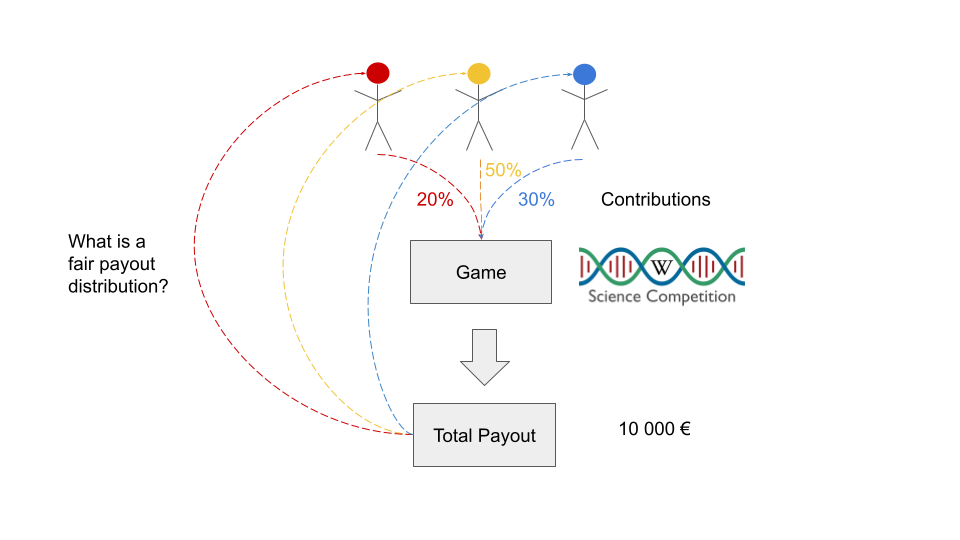
\includegraphics{figure/Shapley_1.png}
% \end{figure}
% \end{frame}

% \begin{frame}{Fair Payouts are Trivial Without Interactions}
% \begin{figure}
%     \centering
%     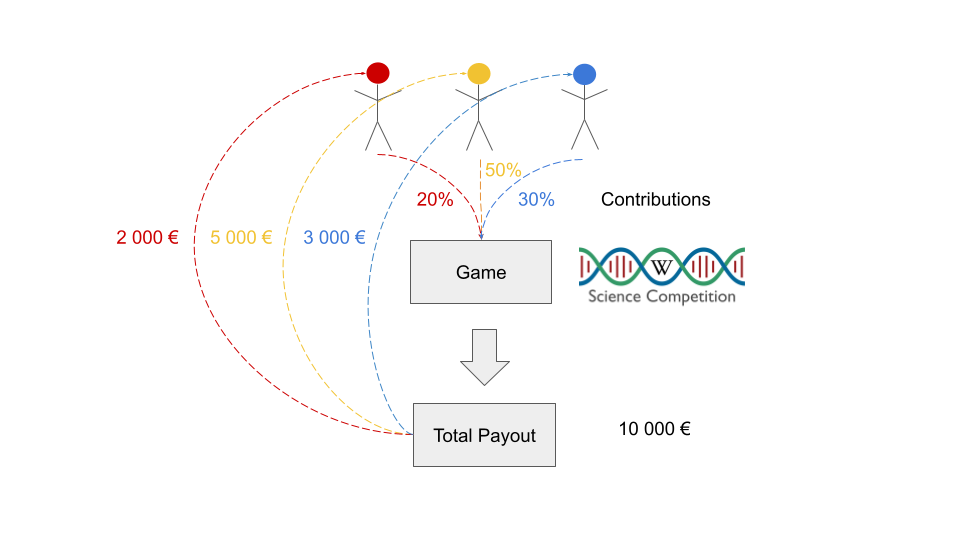
\includegraphics{figure/Shapley_2.png}
% \end{figure}

% \end{frame}
% \begin{frame}{Cooperative Games with Interactions}
% \begin{figure}
%     \centering
%     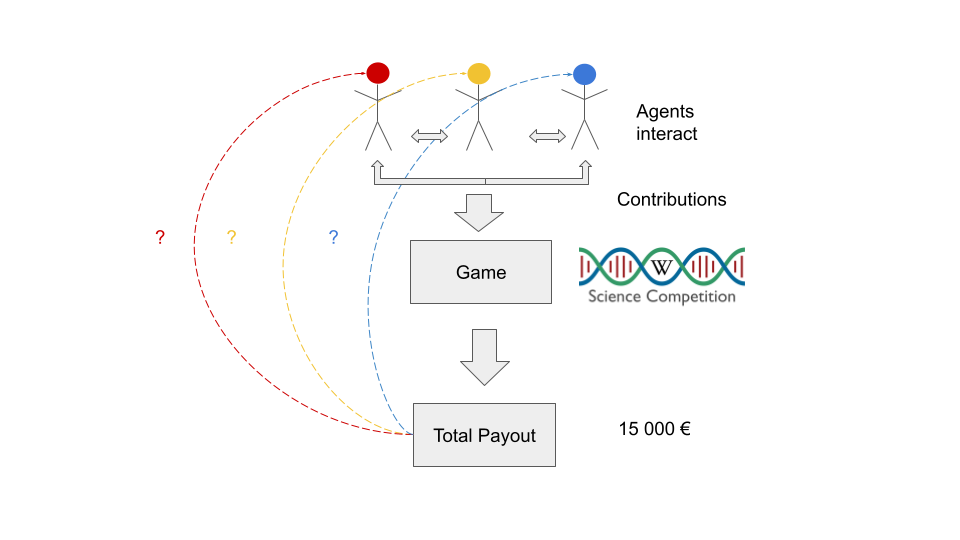
\includegraphics{figure/Shapley_3.png}
% \end{figure}
%\end{frame}

% \begin{frame}{What is a fair payout for player \enquote{yellow}?}

% \begin{figure}
%     \centering
%     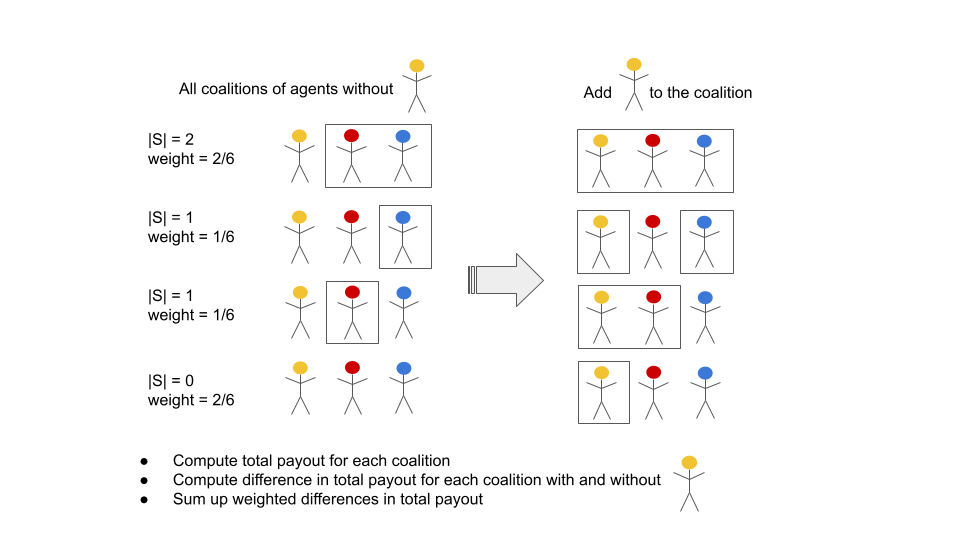
\includegraphics{figure/Shapley_4.png}
% \end{figure}

% \end{frame}



\begin{frame}{Shapley Value - Set definition}

This idea refers to the \textbf{Shapley value} which assigns a payout value to each player according to its marginal contribution in all possible coalitions.
% which  provide a unique solution for the payout attribution problem.
  
\begin{itemize}[<+->]
  %\item Shapley values were proposed by Lloyd Shapley in 1951 for cooperative games (game theory).
  % given axioms of efficiency, symmetry, dummy and additivity.
  %\item The \textbf{Shapley value} of player $j$ assigns a payout value according to the marginal contribution of each player in all possible coalitions\\
  %$\leadsto$ %To compute the Shapley payout for a player $j$, we 
  \item Let $v(\Scupj) - v(S)$ be the marginal contribution of player $j$ to coalition $S$\\
  $\leadsto$ measures how much a player $j$ increases the value of a coalition $S$
  \item Average marginal contributions for all possible coalitions $\SsubPnoj$ \\
  $\leadsto$ order of how players join the coalition matters $\Rightarrow$ different weights depending on size of $S$\\
  %$\leadsto$ marginal contributions are weighted differently
  \item Shapley value via \textbf{set definition} (weighting via multinomial coefficient): 
  $$\phi_j = \sum_{\SsubPnoj} \frac{|S|!(|P| - |S| - 1)!}{|P|!}(v(\Scupj) - v(S))$$
    
  %\item Shapley values are the \texthetit{only} solution for the attribution with the specified axioms.
%   \item Equivalent Shapley value definition via \textbf{orders}: $$\phi_j = \frac{1}{|P|!} \sum_{\tau \in \Pi} (v(\Stau \cup \{j\}) - v(\Stau))$$
%     $\leadsto$ $\Pi$: All possible $|P|!$ orders/permutations of players\\
%     $\leadsto$ $\Stau$: The set of players before player $j$ in order $\tau = (\tau^{(1)}, \dots, \tau^{(p)})$ % j, \dots, 
\end{itemize}

\end{frame}

\begin{frame}{Shapley Value - Mulinomal coefficent intuition}
\[
\frac{|S|!(|P| - |S| - 1)!}{|P|!}
\]
  \item The coefficient tells us the probability that, when randomly arranging all $|P|$ players, the exact set $S$ appears before player $j$, and the remaining players appear afterward.
\centerline{
  \begin{tabular}{|c|c|c|c|c|c|c|}
    \multicolumn{3}{c}{\enspace\raisebox{-3.3ex}[0pt][2.6ex]{$ \overbrace{\vphantom{-}\hspace{9em}}^{|S|! \text{ permutations}}$}} &
    \multicolumn{1}{c}{\enspace\raisebox{-3.3ex}[0pt][1.1ex]{$ \overbrace{\vphantom{-}\hspace{3em}}^{\text{player } j}$}} &
    \multicolumn{3}{c}{\enspace\raisebox{-3.3ex}[0pt][2.6ex]{$ \overbrace{\vphantom{-}\hspace{9em}}^{(|P| - |S| - 1)! \text{ permutations}}$}}\\
    \hline
    $\tau^{(1)}$ & \ldots & $\tau^{(|S|)}$ & $\tau^{(|S| + 1)}$ & $\tau^{(|S| + 2)}$ & \ldots & $\tau^{(|P|)}$ \\
    \hline
  \end{tabular}}

\pause
\begin{figure}[h!]
    \centering
    % code for the figure (https://colab.research.google.com/drive/1kOEZkT2jgjgaK9OFRbnfx8-_C8z7t8v3?usp=sharing)
    \begin{minipage}[b]{0.4\textwidth}
        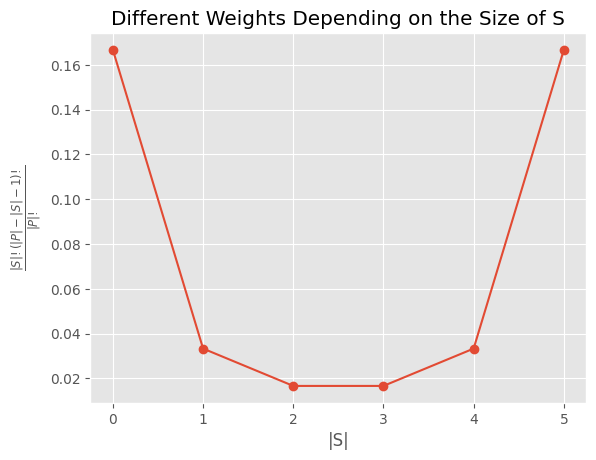
\includegraphics[width=\textwidth]{figure_man/multinom_coef_over_size.png}
    \end{minipage}
    \hspace{0.05\textwidth} 
    \begin{minipage}[b]{0.5\textwidth}
        \small
        \begin{itemize}
          \item Joining early yields a larger weight, because it is harder to contribute when the coalition is still small.
          \item Joining last can also lead to a high weight, since it is challenging to add value to an almost-complete coalition.
          \item Being in the middle results in a lower weight.
        \end{itemize}
    \end{minipage}
\end{figure}
\end{frame}

% \begin{frame}{How to Weight Differences in Payout?}

% \begin{itemize}
%     %\itemsep2em
%     %\item Form a coalition one player at a time -- each player receives its contribution to the total payout, i.e., the increase in total payout when a player joins a coalition
%     % \item The Shapley value is the players' average contribution over all possible formations of coalitions\\
%     % $\leadsto$ order of how players join the coalition matters\\
%     % $\leadsto$ marginal contributions are weighted
%     %\item Each contribution is weighted proportionally to the number of possible orders of its coalition -- the more players in a coalition, the more possibilities of ordering the players inside the coalition
%     \item Shapley value via \textbf{set definition} (weighting via multinomial coefficient): 
%     $$\phi_j = \sum_{\SsubPnoj} \frac{|S|!(|P| - |S| - 1)!}{|P|!}(v(\Scupj) - v(S))$$
%     \item Shapley value via \textbf{order definition}: $$\phi_j = \frac{1}{|P|!} \sum_{\tau \in \Pi} (v(\Stau \cup \{j\}) - v(\Stau))$$
    
%     with $\Pi$ being all possible $|P|!$ orders/permutations of players and $\Stau$ being the set of players before player $j$ in order $\tau$ 
    
%     %$\phi_j = \frac{1}{|P|!} \sum_{\tau \in \Pi} (v(S_j(\tau) \cup \{j\}) - v(S_j(\tau)))$
% \end{itemize}

% \end{frame}

% \begin{frame}{How to Weight Differences in Payout?}

% \begin{figure}
%     \centering
%     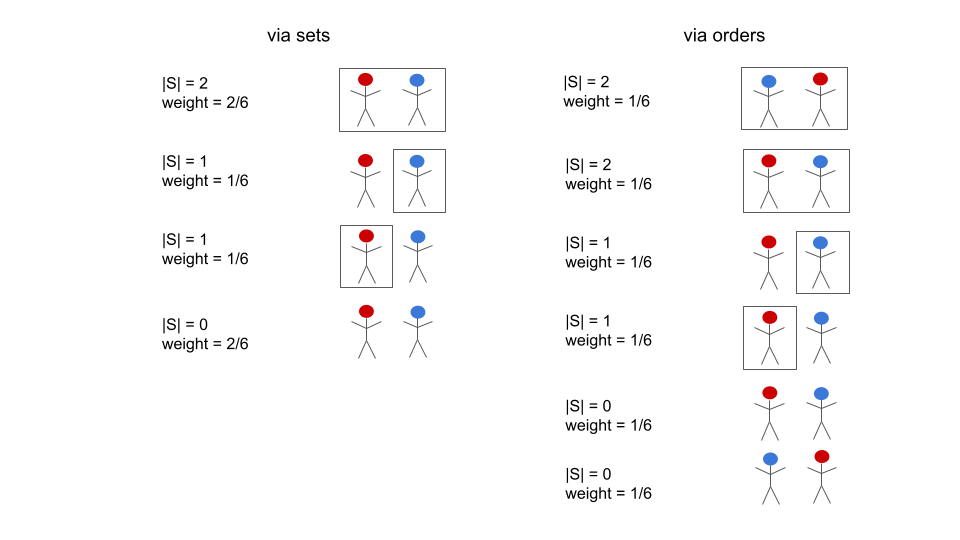
\includegraphics{figure/Shapley_5.png}
% \end{figure}

% \end{frame}



% \begin{frame}{From Game Theory To Machine Learning}

% \begin{figure}
%     \centering
%     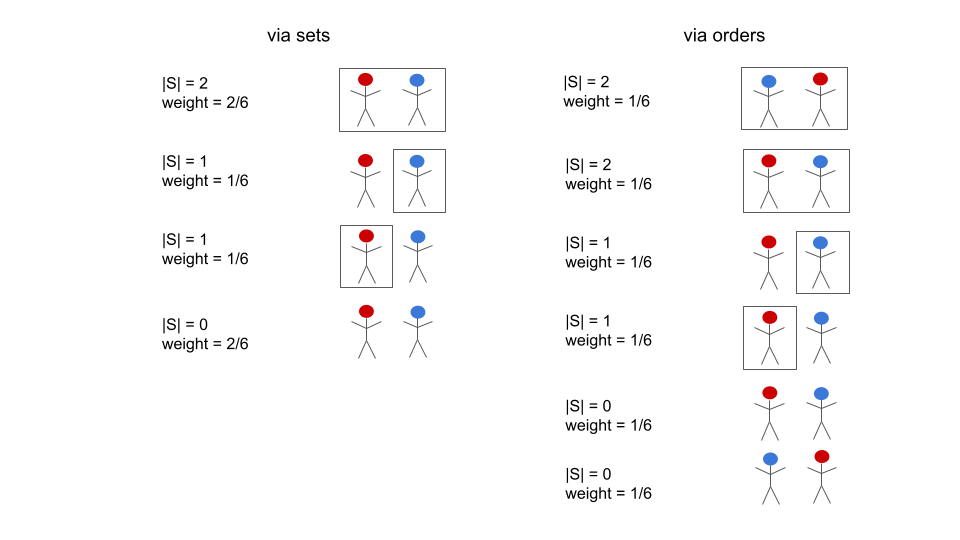
\includegraphics{figure/Shapley_5.png}
% \end{figure}

% \end{frame}

% \begin{frame}{Shapley Values}

%   Shapley values provide a unique solution to the attribution problem while satisfying all axioms:
%     \vspace{0.25cm}
% \begin{itemize}
%   \itemsep1em
%   \item Shapley values were proposed by Lloyd Shapley in 1951.
%   \item The Shapley value assigns a value to each player according to the marginal contribution of each player in all possible coalitions.
%   \item $\phi_j = \sum_{\SsubPnoj} \frac{|S|!(|P| - |S| - 1)!}{|P|!}(v(\Scupj) - v(S))$
%   \item $v(\Scupj) - v(S)$ is the marginal contribution of player $j$ to coalition $S$.
%   \item To compute the Shapley payout for a player, we average, for all possible coalitions, how much the player would increase the value of the coalition (=marginal contribution).
%   \item Shapley values are the \textit{only} solution for the attribution with the specified axioms.
% \end{itemize}

% \footnote{Shapley, Lloyd S. (August 21, 1951). "Notes on the n-Person Game -- II: The Value of an n-Person Game" (PDF). Santa Monica, Calif.: RAND Corporation.}

% \end{frame}



\begin{frame}{Shapley Value - Order Definition}
The Shapley value was introduced as summation over sets $\SsubPnoj$, but it can be equivalently defined as a summation of all orders of players: 
%(which explains where the factor $\frac{|S|!(|P| - |S| - 1)!}{|P|!}$ comes from):

$$\phi_j = \frac{1}{|P|!} \sum_{\tau \in \Pi} (v(\Stau \cup \{j\}) - v(\Stau))$$
  
\begin{itemize}[<+->]
  \item $\Pi$: All possible orders of players (we have $|P|!$ in total)
  %\item Recall the order definition: 
  \item $\Stau$: Set of players before player $j$ in order $\tau = (\tau^{(1)}, \dots, \tau^{(p)})$  where $\tau^{(i)}$ is $i$-th element \\ % j, \dots, 
  $\Rightarrow$ Example: Players $1,2,3$ $\Rightarrow$ 
  \only<3>{$\Pi = \{({\color{red} 1,2},3), (1,3,2), ({\color{red} 2,1},3), (2,3,1), (3,1,2), (3,2,1)\}$}%
  \only<1-2>{$\Pi = \{(1,2,3), (1,3,2), (2,1,3), (2,3,1), (3,1,2), (3,2,1)\}$}%
  \\
  \phantom{$\Rightarrow$} $\leadsto$ For order $\tau = (2,1,3)$ and player of interest $j=3$ $\Rightarrow$ $\Stau = \{2, 1\}$\\
  \phantom{$\Rightarrow$} $\leadsto$ For order $\tau = (3,1,2)$ and player of interest $j=1$ $\Rightarrow$ $\Stau = \{3\}$\\
  \phantom{$\Rightarrow$} $\leadsto$ For order $\tau = (3,1,2)$ and player of interest $j=3$ $\Rightarrow$ $\Stau = \emptyset$
  %\item In order definition, we sum the marginal contribution twice for orders that yield set $S = \{1,2\}$\\
  \item Order definition: Marginal contribution of orders that yield set {\color{red} $S = \{1,2\}$} is summed twice\\
  $\leadsto$ In set definition, it has the weight $\tfrac{2! (3 - 2 - 1)!}{3!} = \tfrac{2 \cdot 0!}{6} = \tfrac{2}{6}$
\end{itemize}

\end{frame}


\begin{frame}{Shapley Value - Comments on Order Definition}

\begin{itemize}
  \item<1-> Order and set definition are equivalent
  \item<1-> Reason: The number of orders which yield the same coalition $S$ is $|S|!(|P| - |S| - 1)!$\\
  $\Rightarrow$ There are $|S|!$ possible orders of players within coalition $S$\\
  $\Rightarrow$ There are $(|P| - |S| - 1)!$ possible orders of players without $S$ and $j$
  \centerline{
  \begin{tabular}{|c|c|c|c|c|c|c|}
    \multicolumn{3}{c}{\enspace\raisebox{-3.3ex}[0pt][2.6ex]{$ \overbrace{\vphantom{-}\hspace{9em}}^{|S|! \text{ permutations}}$}} &
    \multicolumn{1}{c}{} &
    \multicolumn{3}{c}{\enspace\raisebox{-3.3ex}[0pt][2.6ex]{$ \overbrace{\vphantom{-}\hspace{9em}}^{(|P| - |S| - 1)! \text{ permutations}}$}}\\
    \hline
    $\tau^{(1)}$ & \ldots & $\tau^{(|S|)}$ & $\tau^{(|S| + 1)}$ & $\tau^{(|S| + 2)}$ & \ldots & $\tau^{(p)}$ \\
    \hline
    \multicolumn{3}{c}{\enspace\raisebox{1.3ex}[0pt][2.6ex]{$ \underbrace{\vphantom{-}\hspace{9em}}^{}$}} &
    \multicolumn{1}{c}{\enspace\raisebox{1.3ex}[0pt][2.6ex]{$ \underbrace{\vphantom{-}\hspace{4em}}^{}$}} &
    \multicolumn{3}{c}{\enspace\raisebox{1.3ex}[0pt][2.6ex]{$ \underbrace{\vphantom{-}\hspace{9em}}^{}$}}\\
    \multicolumn{3}{c}{Players before player $j$} & \multicolumn{1}{c}{player $j$} & \multicolumn{3}{c}{Players after player $j$} \\
  \end{tabular}}
  \item<2-> Relevance of the order definition: Approximate Shapley values by sampling permutations \\
  $\leadsto$ randomly sample a fixed number of $M$ permutations and average them:
  %to approximate the Shapley values
  %instead of producing all $|P|!$ permutations, a fixed number of $M< |P|!$ permutations can be sampled and averaged to approximate the Shapley values
  $$\phi_j = \frac{1}{M} \sum_{\tau \in \Pi_M} (v(\Stau \cup \{j\}) - v(\Stau))$$
    where $\Pi_M \subset \Pi$ is a random subset of $\Pi$ containing only $M$ orders of players\\
    %$\leadsto$ $\Stau$: For permutation $\tau$, the set of players before player $j$ in order $\tau$ 
\end{itemize}

\end{frame}


% How to weight differences in payout
\begin{frame}{Weights for Marginal Contribution - Illustration}
%   \begin{center}
%   \only<1>{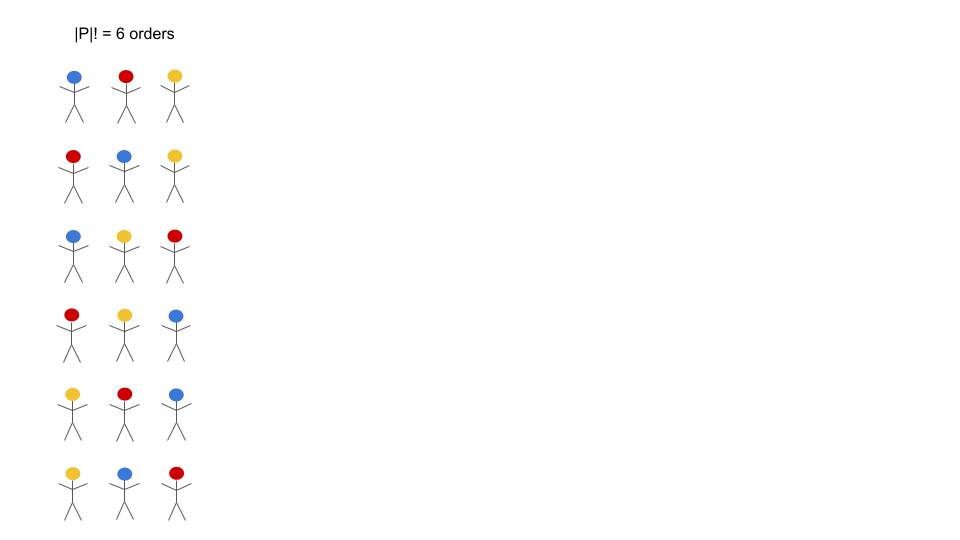
\includegraphics{figure/Shapley_7.png}}%
%   \only<2>{ 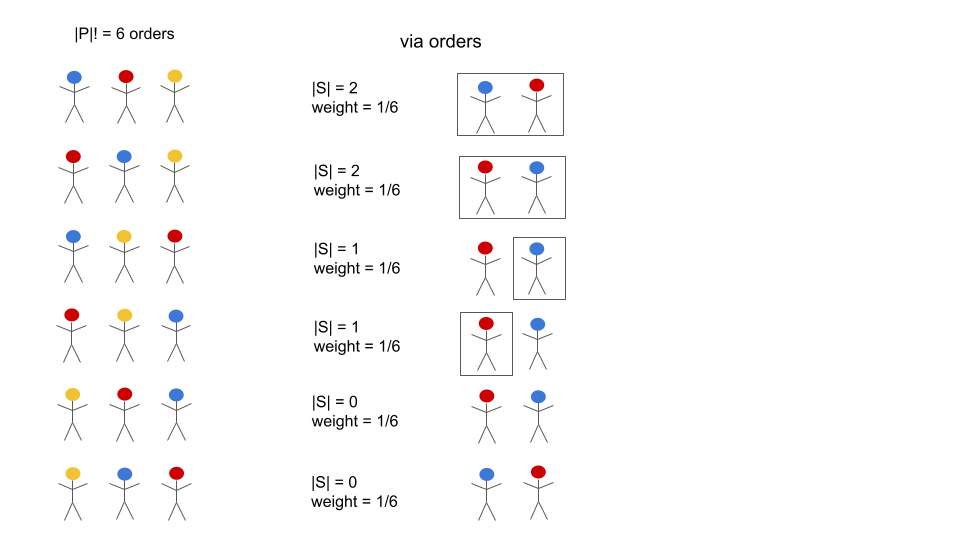
\includegraphics{figure/Shapley_8.png}}%
%   \only<3>{ 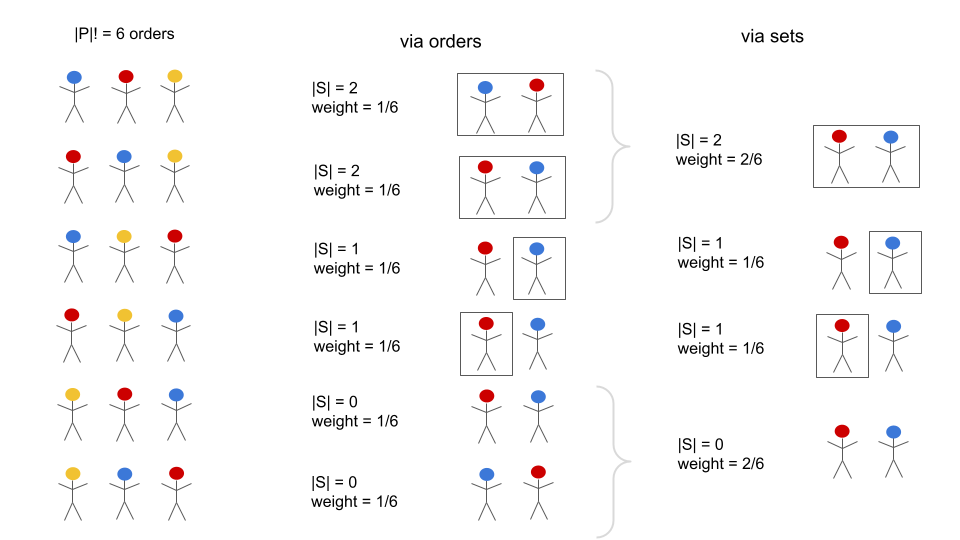
\includegraphics{figure/Shapley_9.png}}%
%   \end{center}
  
\begin{center}
\includegraphics<1>[page=5, width = 0.8\textwidth]{figure/Shapley.pdf}%
\includegraphics<2>[page=6, width = 0.8\textwidth]{figure/Shapley.pdf}%
\includegraphics<3>[page=7, width = 0.8\textwidth]{figure/Shapley.pdf}%
\end{center}
\end{frame}


\begin{frame}{Shapley Values - Illustration}
\begin{itemize}
    \item Shapley value of player $j$ is the marginal contribution to the value when it enters any coalition
    \item Produce all possible joining orders of player coalitions
%\only<1>{\item Here, player $2$ enters the coalition after player $1$, resulting in a value change of $v(\{1,2\}) - v(\{1\}) = 24-12 = 12$ with a overall coalition value of $v(\{1,2,3\}) = 36$}
\only<1>{\item[] \phantom{Measure and average the difference in payout after player $1$ enters the coalition}}%
\only<2>{\item Measure and average the difference in payout after player $1$ enters the coalition}%
\only<3>{\item Measure and average the difference in payout after player $2$ enters the coalition}%
\only<4>{\item Measure and average the difference in payout after player $3$ enters the coalition}%
\end{itemize}

\begin{center}
\includegraphics<1>[page=9, width = 0.7\textwidth]{figure/Shapley.pdf}%
\includegraphics<2>[page=10, width = 0.7\textwidth]{figure/Shapley.pdf}%
\includegraphics<3>[page=11, width = 0.7\textwidth]{figure/Shapley.pdf}%
\includegraphics<4>[page=12, width = 0.7\textwidth]{figure/Shapley.pdf}%
\includegraphics<5>[page=13, width = 0.7\textwidth]{figure/Shapley.pdf}%
\end{center}

% \begin{center}
%   \only<1>{
%     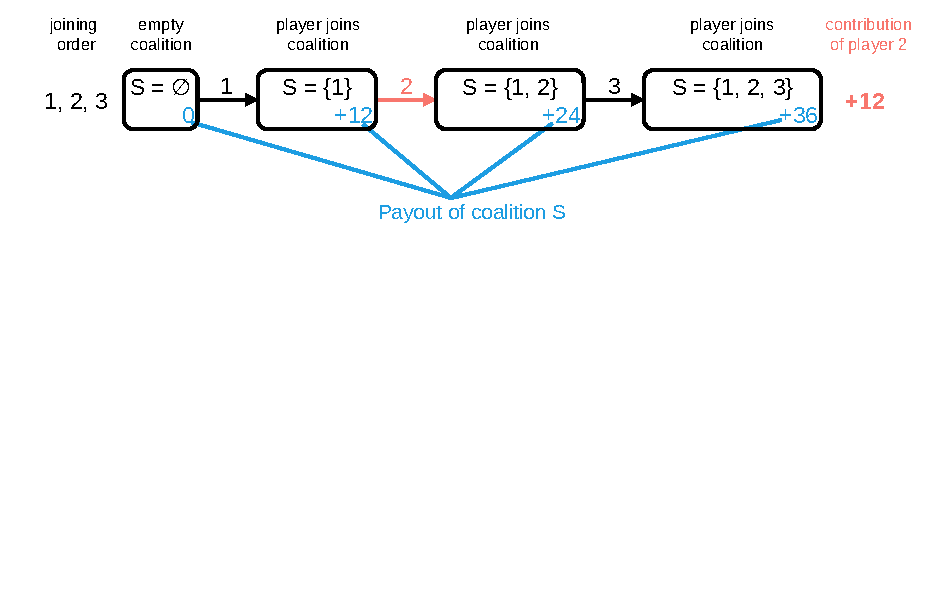
\includegraphics[page=1, width=0.6\textwidth]{figure_man/shapley_feature_effect}
%   }
%   \only<2>{
%     \includegraphics[page=2, width=0.6\textwidth]{figure_man/shapley_feature_effect}
%   }
% \end{center}
\end{frame}


\begin{frame}{Axioms of Fair Payouts}
 Why is this a fair payout solution?
 \\
 One possibility to define fair payouts are the following axioms for a given value function $v$:
  \vspace{0.25cm}
  \begin{itemize}[<+->]
  \itemsep1em
    \item \textbf{Efficiency}: Player contributions add up to the total payout of the game:
      $\sum\nolimits_{j=1}^p\phi_j = v(P)$
    % symmetry - "any" confused me a bit since we actually look into coalitions that do not include both j and k. Maybe we can state this more as "for any coalition it make no difference whether we add $j$ or $k$"
    \item \textbf{Symmetry}: Players $j,k \in P$ who contribute the same to any coalition get the same payout: \\ 
      If $v(\Scupj) = v(\Scupk)$ for all $\SsubP \setminus\{j,k\}$, then $\phi_j=\phi_k$
    \item \textbf{Dummy/Null Player}: Payout is 0 for players who don't contribute to the value of any coalition: \\
      If $v(\Scupj)=v(S)\quad  \forall \quad \SsubP \setminus \{j\}$, then $\phi_j=0$
    \item \textbf{Additivity}: For a game $v$ with combined payouts $v(S) = v_1(S) + v_2(S)$, the payout is the sum of payouts: $\phi_{j,v} = \phi_{j,v_1} + \phi_{j, v_2}$
  \end{itemize}
  \vspace{0.5cm}
  

\end{frame}

% \begin{frame}{Proof of Axioms}
%   The Shapley values fulfills all the 4 axioms.
%   Symmetry, Dummy and Additivity are relatively easy to proof:
% \begin{itemize}
%     % See also: https://math.stackexchange.com/questions/2747088/shapley-value-is-efficient
%   \item \textbf{Symmetry}: Let's assume coalition $\SsubPnojk$ and $v(\Scupj) = v(\Scupk)$.
%     \begin{itemize}
%         \item Then all marginal contributions are equal: $v(\Scupj) -  v(S) = v(\Scupk) -  v(S), \forall \SsubPnojk$
%         \item Consequently, $\phi_j = \phi_k$.
%     \end{itemize}
%   \item \textbf{Dummy}: Let's assume we have player $j$ such that for all $\SsubP$, we have $v(S) = v(\Scupj)$. Then, each marginal contribution of player $j$ is zero, and therefore $\phi_j = 0$.
%   \item \textbf{Additivity}:  Assume two games $v_1$ and $v_2$ and a third game which is the sum of both $v(S) = v_1(S) + v_2(S)$. The marginal contribution for all $\SsubPnoj$ for game $v$ can be expressed as $v(\Scupj) - v(S) = v_1(\Scupj) - v_1(S) + v_2(\Scupj) - v_2(S)$. Since the Shapley value is additive in the marginal contributions, we can split the sum into two sums so that $\phi_{j,v} = \phi_{j, v_1} + \phi_{j,v_2}$.
% \end{itemize}
% Efficiency requires a bit more effort, see proof sketch:
%   \begin{itemize}
%   \item \textbf{Efficiency}: $v(P)$ exactly appears once per player ($=p$ times) for coalition $S = P \setminus \{j\}$ with the weight $\frac{|P - 1|!(|P| - |P - 1| - 1)!}{|P|!} = \frac{1}{p}$ each. The values for all other coalitions $v(S), \SsubP \{j,k\}$ appear with both minus and plus signs that cancel each other out.
% \end{itemize}
% \end{frame}


% \begin{frame}{Linearity Axiom Corollary}
%   \begin{itemize}
%   \item The Shapley values are also linear:
%   \item For a game with payout $v(S) = \alpha v_1(S) + v_2(S)$, the Shapley values are $\alpha \phi_{j,v_1} + \phi_{j,v_2}$.
%   \item The multiplication with $\alpha$ works since we can pull out $\alpha$ from the sum of marginal contributions, so that for $v(S) = \alpha v_1(S)$ the Shapley value is $\alpha \phi_{j,v_1}$.
%   \item We already know that Shapley values are additive which proofs the linearity.
%   \end{itemize}
% \end{frame}



% \begin{frame}{Applications of Shapley Value}

%   \begin{itemize}
%       \item Game theory
%       \item Economics (e.g., cost allocation)
%       \item Marketing (e.g., social network analysis to discover influencers)
%       \item ...
%       \item Machine learning
%       \begin{itemize}
%          \item Feature selection: Attribute loss reduction to features.
%          \item Quantify data value: Attribute loss reduction to data points.
%          \item \textbf{Explain individual predictions}.
%       \end{itemize}
%   \end{itemize}

%   % Economics
%   \tiny{Moulin, Hervé. "An application of the Shapley value to fair division with money." Econometrica: Journal of the Econometric Society (1992): 1331-1349.}
% % Network analysis
%   \tiny{Narayanam, Ramasuri, and Yadati Narahari. "A shapley value-based approach to discover influential nodes in social networks." IEEE Transactions on Automation Science and Engineering 8.1 (2010): 130-147.}
%   % Feature Selection
%   \tiny{Cohen, Shay B., Eytan Ruppin, and Gideon Dror. "Feature Selection Based on the Shapley Value." IJCAI. Vol. 5. 2005.}
%   % Value of data
%   \tiny{Ghorbani, Amirata, and James Zou. "Data shapley: Equitable valuation of data for machine learning." International Conference on Machine Learning. PMLR, 2019.}
% \end{frame}

\endlecture
\end{document}
